\chapter{Verwandte Themen}\label{ch:related}
Im Netzwerk AMBIENCE, das als Schnittstelle für den eigenen Entwurf diente, spielen Bloom-Filter eine wichtige Rolle. Für die vorliegende Arbeit wurden die Bloom-Filter jedoch selbst implementiert, um eigene Berechnungen zu überprüfen und mit realistischen Werten arbeiten zu können. Das folgende Kapitel stellt in Abschnitt \ref{sec:bloom-implementierung} zunächst dar, auf welche Arbeiten und bewährten Techniken dabei Bezug genommen wurde. 

Ziel dieser Arbeit war eine optimale Lösung für das Anwendungsszenario von AMBIENCE. Eine solche wird vom aktuellen Stand der Forschung nicht abgedeckt. Die Darstellung des aktuellen Forschungsstandes konzentriert  sich wegen der Fülle der Einsatzmöglichkeiten auf Bloom-Filter in Netzwerkanwendungen und Indexstrukturen sowie die \textit{k}-nächste-Nachbarn-Suche. Überlegungen und Arbeiten, die Eingang in die eigene Implementierung gefunden haben, werden in den Abschnitten \ref{sec:bloom-netzwerk}, \ref{sec:bloom-index} und \ref{sec:bloom-knn} vorgestellt. 
\section{Einsatz von Bloom-Filtern}\label{sec:bloom-implementierung}
Gemäß dem Bloom-Filter-Prinzip bietet sich die Verwendung von Bloom-Filtern an, wenn Speicherplatz effektiv genutzt werden soll und gleichzeitig die Auswirkungen von falsch positiven Ergebnissen abgemildert werden können (vgl. Abschnitt \ref{sec:bloom-anwendungen}). Die mathematischen Grundlagen wie Minimierung der Falsch-Positiv-Rate, Abschätzung der Anzahl eingefügter Elemente, Abschätzung der Jaccard-Distanz etc. werden beispielsweise von Bloom \cite{Bloom1970}, Broder \cite{Broder2004}, Mitzenmacher \cite{Mitzenmacher2002} sowie Werner et al. \cite{Werner2015} ausführlich dargestellt. 

Wie in den Abschnitten \ref{sec:hashfunktionen} und \ref{sec:bloom-anwendungen} erwähnt, werden Bloom-Filter im Apache-Projekt Cassandra eingesetzt. Sie dienen dort zum schnellen Nachschlagen in Tabellen, den so genannten \textit{SSTables}. Die Cassandra-Entwickler, namentlich Jonathan Ellis, haben sich eingehend mit der Implementierung von Bloom-Filtern und optimalen Hashfunktionen beschäftigt. Diese Überlegungen haben keinen Eingang in wissenschaftliche Veröffentlichungen gefunden, sind jedoch sehr praxisrelevant\footnote{Die Hauptseite des Cassandra-Projekts ist unter \url{http://cassandra.apache.org/} (17.07.2016) zu finden. Der Cassandra-Quellcode ist frei verfügbar unter \url{https://github.com/apache/cassandra} (17.07.2016). Datenmodell und Architektur werden z.B. unter \url{http://wiki.apache.org/cassandra/DataModel} (17.06.2016), \url{http://wiki.apache.org/cassandra/ArchitectureOverview} (17.07.2016) und \url{http://prettyprint.me/prettyprint.me/2010/05/02/understanding-cassandra-code-base/index.html} (17.07.2016) beschrieben. Für diese Arbeit wurden auch eine  programmatische Rede unter \url{https://youtu.be/WD1v6jr5fKY} (17.07.2016) und ein Blog unter \url{http://spyced.blogspot.de/} (17.07.2016) von Ellis berücksichtigt.}. Zur Wahl der Hashfunktionen schreibt Ellis: 
% \newpage
\begin{quote}
\textit{"`[I]t turns out that it's surprisingly hard to find good information on one part of the implementation: how do you generate an indefinite number of hashes? Even small filters will use three or four; a dozen or more is not unheard of."'}\footnote{\mbox{\url{http://spyced.blogspot.de/2009/01/all-you-ever-wanted-to-know-about.html} (17.07.2016).}} 
\end{quote}
Die mathematischen Grundlagen der Generierung von \textit{i} Hashfunktionen mit möglichst gleich verteilten Ergebnissen sind bei Kirsch und Mitzenmacher zu finden \cite{Kirsch2006}. Viele Bloom-Filter-Implementierungen wie \textit{PyBloom} verwenden jedoch Hashfunktionen, deren Ergebnisse nicht gleich verteilt sind. Das Problem ist, dass damit häufig eine deutlich höhere Falsch-Positiv-Rate im Bloom-Filter erzielt wird als rein rechnerisch zu erwarten wäre. 

Der Grund für die Verwendung minderwertiger Hashfunktionen ist Ellis zu Folge, dass die meisten Implementierungen auf schnelle Berechnung der Hashwerte abzielten statt auf Gleichverteilung der Ergebnisse. Das ist aber für einen Bloom-Filter essentiell, wenn z.B. wie in Cassandra teure Eingabe/Ausgabe-Operationen durch den Einsatz von Bloom-Filtern reduziert werden sollen. Weist der Bloom-Filter eine erhöhte Falsch-Positiv-Rate auf, beispielsweise von 140\% gegenüber dem erwarteten Wert, reduziert das die positiven Effekte des Bloom-Filters drastisch.  

Ellis präsentiert zwei Lösungsansätze: Entweder kryptografische Hashfunktionen oder Murmur- und Jenkins-Hashfunktionen mit guter Gleichverteilung der Ergebnisse. Kryptografische Hashfunktionen wurden bereits in Abschnitt \ref{sec:hashfunktionen} dargestellt. Der Nachteil daran ist, dass sie in der Regel aufwändiger zu berechnen sind als gewöhnliche Hashfunktionen. Das spielt z.B. bei der einmaligen Berechnung eines Fingerabdrucks keine große Rolle. Die Performanz von Bloom-Filtern wird dadurch aber beeinträchtigt. 

Mit Murmur- oder Jenkins-Hashfunktionen gibt es zwei Möglichkeiten, eine beliebige Anzahl von Hashfunktionen mit guter Gleichverteilung der Ergebnisse zu erzeugen. Entweder berechnet man den \textit{i}-ten Hashwert als $\text{hash0 }+ i\ast \text{hash1}$ wie von Kirsch und Mitzenmacher beschrieben und in Cassandra angewendet. Alternativ nimmt man den \textit{i}-ten Hashwert als Startwert für die Berechnung des \textit{i+1}-ten Hashwerts. Dieser Ansatz wurde in Hadoop gewählt und wird auch hier verwendet. 

Zur Organisation der Bloom-Filter äußert sich Ellis ebenfalls, jedoch nur auf seinem Twitter-Account und ohne auf Details einzugehen: 
\begin{quote}
\textit{"`Rather than naively checking every Bloom Filter for the element, organize the BF in a hierarchy akin to B+ tree."'}\footnote{\url{https://twitter.com/spyced/status/707266703751651328} (17.07.2016).}
\end{quote}
Zwar ist hier offensichtlich von der Suche nach einem Element in einem Bloom-Filter die Rede, nicht nach einem Bloom-Filter selbst wie in AMBIENCE. Dennoch zeichnet sich ab, dass ein B$^+$-Baum als Indexstruktur für Bloom-Filter in Erwägung gezogen werden sollte. 

Damit sind die Gemeinsamkeiten zwischen Cassandra und AMBIENCE erschöpft. Cassandra ist zur Evaluation von AMBIENCE nicht geeignet, da in AMBIENCE die Bloom-Filter selbst die Datensätze sind, während sie in Cassandra zum Nachschlagen der Datensätze verwendet werden. Die Publikationen aus dem Cassandra-Umfeld wurden daher ausschließlich bezüglich Implementierung der Bloom-Filter, Wahl und Berechnung der Hashfunktionen berücksichtigt. Der Hinweis auf B$^+$-Bäume in Zusammenhang mit Bloom-Filtern unterstützte zudem die Entscheidung für diese Indexstruktur. 
\section{Netzwerkanwendungen mit Bloom-Filtern}\label{sec:bloom-netzwerk}
Bloom-Filter werden in zahlreichen Netzwerk-Anwendungen eingesetzt. Das erscheint auf den ersten Blick interessant für AMBIENCE als soziales Online-Netz. Ein guter Überblick über Netzwerk-Anwendungen mit Bloom-Filtern findet sich in der Publikation von Broder und Mitzenmacher mit dem Ziel 
\begin{quote}
\textit{"`[...] to survey the ways in which Bloom filters have been used and modified in a variety of network problems, with the aim of providing a unified mathematical and practical framework for understanding them and stimulating their use in future applications."'} \cite{Broder2004}
\end{quote}
Die Autoren beschreiben unter anderem die Verwendung von Bloom-Filtern zur Kollaboration in Overlay- und Peer-to-Peer-Netzwerken, jedoch mit einem entscheidenden Unterschied zur Fragestellung: Zwar werden die Anfragen in AMBIENCE von einem mobilen Endgerät an einen Host gesendet, also über das Netzwerk übertragen. Die \textit{k}-nächste-Nachbarn-Suche bezieht sich jedoch auf die Menge der an einem Host gespeicherten Bloom-Filter. Unter diesen sollen die ähnlichsten möglichst schnell und effizient gefunden werden. Ab dem Zeitpunkt, zu dem die Anfrage am Host eingegangen ist, werden aber keine Nachrichten mehr im Netzwerk übertragen. Die \textit{k}-nächste-Nachbarn-Suche findet nur auf dem Host selbst statt und erst das Ergebnis wird an das anfragende Gerät übermittelt. 

Ähnlich verhält es sich mit der Arbeit von Agarwal und Trachtenberg. Dort werden Counting Bloom-Filter verwendet, um die Abschätzung von Mengendifferenzen auf unterschiedlichen Hosts zu optimieren \cite{Agarwal2006}. Daran werden zwar die Vorteile von Bloom-Filtern bei der blinden Kalkulation von Mengenunterschieden deutlich, ohne dass ihre Elemente bzw. die Objekte in den Bloom-Filtern bekannt sein müssen. Wie bei Werner et al. beschrieben, kann diese Eigenschaft den Schutz der Privatsphäre in einem sozialen Online-Netz verbessern \cite{Werner2015}. Auch hier findet die Abschätzung der Mengendifferenzen jedoch zwischen zwei unterschiedlichen Hosts statt, weswegen dieser Ansatz für AMBIENCE nicht genutzt werden kann. Gleiches gilt für die Arbeiten von Byers et al. \cite{Byers2002}, Shiraki et al. \cite{Shiraki2009}, Zhang \cite{Zhang2012} und Zhu et al. \cite{Zhu2004}. Überall dort werden Bloom-Filter im Zusammenhang mit Netzwerken eingesetzt, doch keiner der Ansätze lässt sich auf AMBIENCE anwenden. 
\section{Indexstrukturen für Bloom-Filter}\label{sec:bloom-index}
Ein Überblick über Indexstrukturen für Datenbank-Managementsysteme auf Hauptspei\-cher\-basis findet sich bei Lehman und Carey \cite{Lehman1986}. Die Publikation kann zu einem besseren Verständnis der Indexstrukturen aus Abschnitt \ref{sec:indexstrukturen} beitragen. Wichtig ist vor allem die Erkenntnis, dass der Einsatz einer Hauptspeicher-Datenstruktur sinnvoll sein kann, um die Performanz von Anfragen auf größeren Datenmengen zu verbessern. B- und B$^+$-Bäume werden allgemein als Hauptspeicher-Datenstruk\-turen verwendet. Ein Vorteil davon ist die Reduzierung der Plattenzugriffe bei der Suche nach Datensätzen. In der Regel benötigen sie viel weniger Speicherplatz als das tatsächliche Datenaufkommen. Außerdem kann in der Indexstruktur häufig mit Zeigern gearbeitet werden, ohne alle vorhandenden Daten tatsächlich in der Datenstruktur halten zu müssen. Adaptierungen von kanonischen Formen der Indexstrukturen für spezifische Anwendungen finden sich vielfach in der Literatur. Wenig überraschend ist darunter keine, die das spezifische Szenario von AMBIENCE abbildet.

Hellerstein und Pfeffers Publikation von 1994 stellt den \textit{RD-Tree} als Indexstruktur für objektrelationale Geo-Datenbanken vor \cite{Hellerstein1994}. Abgesehen davon, dass der objektrelationale Ansatz mittlerweile kaum noch verfolgt wird, ist die Indexstruktur optimiert für Geodaten. Diese haben spezielle Eigenschaften wie z.B. Inklusionsbeziehungen zwischen Punkten und Flächen oder Flächen untereinander, die in der Indexstruktur abgebildet und von Suchanfragen unterstützt werden müssen. Spezielle Indexstrukturen für Geodaten erschienen daher ungeeignet, da sie einerseits einen unnötigen Implementierungsaufwand erfordern, der für die vorhandenen Daten nicht erforderlich wäre, andererseits die \textit{k}-nächste-Nachbarn-Suche unnötig erschweren. Zu diesen speziellen Indexstrukturen zählt auch der \textit{R-Baum} zur Organisation von minimalen umgebenden Rechtecken. Eine Variante davon ist der \textit{bichromatic Rdnn-Tree} von der Yang und Lin \cite{Yang2002}. Diese Arbeit erschien insofern interessant, als die Autoren nicht nur Punkt-Anfragen, sondern \textit{k-}nächste-Paare und \textit{k}-nächste-Nachbarn-Paare betrachten und ihre Indexstruktur dafür optimiert haben. Mangels Ähnlichkeit von Bloom-Filtern und spatialen Datensätzen wurde jedoch auch dieser Ansatz verworfen. 

Am stärksten wurde schließlich die Arbeit \textit{Evaluation of the Structured Bloom Filters Based on Similarity} von Hiroshi Sakuma und Fumiaki Sato berücksichtigt \cite{Sakuma2011}. Sie behandelt zwar ein Netzwerk-Problem, doch ließen sich Teile der Indexstruktur für AMBIENCE adaptieren. Kern der Arbeit ist ein Baum aus Bloom-Filtern zur Minimierung der Weiterleitungen von Anfragen in einem Verteilten System. 
\begin{figure}[hpbt]
  \centering
  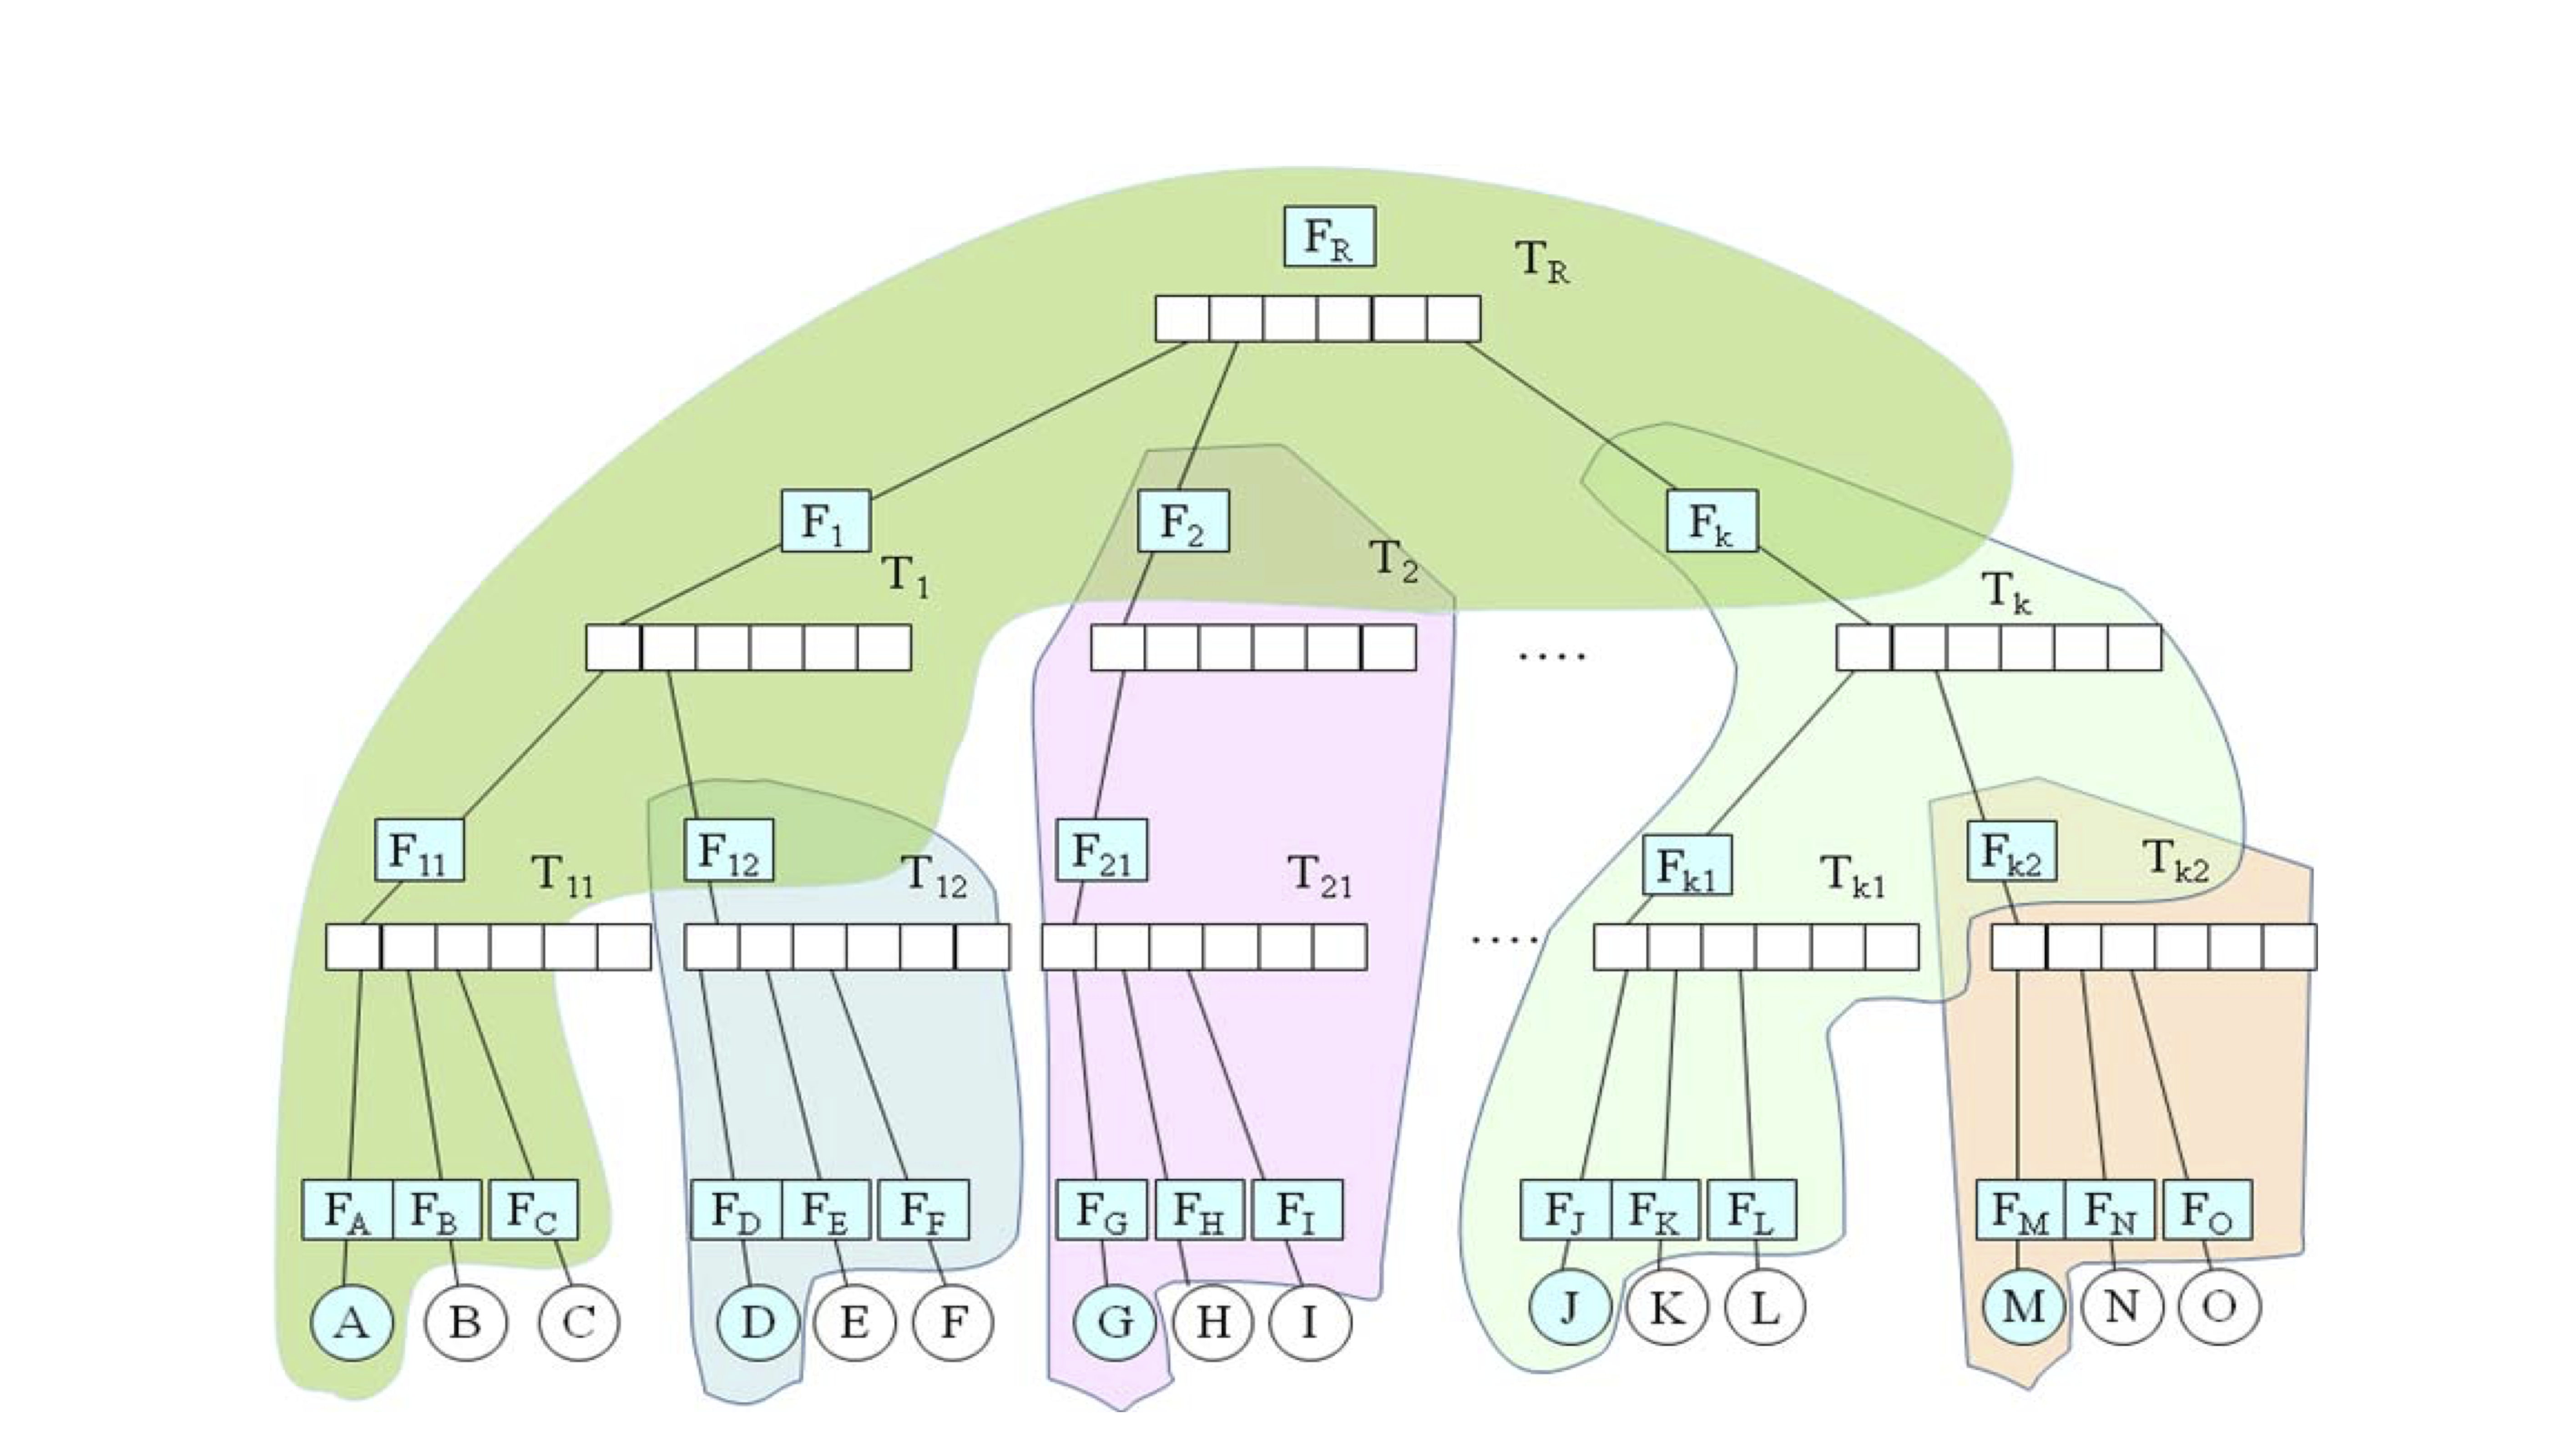
\includegraphics[width=1.0\textwidth]{pictures/bloom-filter-baum.png}\\
  \caption[Bloom-Filter-Baum bei Sakuma und Sato]{Bloom-Filter-Baum bei Sakuma und Sato \cite{Sakuma2011}.}\label{fig:pic5}
\end{figure}
Die Indexstruktur ist ein Baum aus Bloom-Filtern, an dem jeder im Netzwerk beteiligte Knoten einen Teil hält (vgl. Abbildung \ref{fig:pic5}). Er ist nach Ähnlichkeit zwischen Bloom-Filtern aufgebaut. Wie in Abschnitt \ref{sec:distanzmasse} beschrieben, dient als Ähnlichkeitsmaß jedoch nicht die Jaccard-Distanz, sondern die Anzahl gleicher 1-Bits. Die Datensätze werden nicht im Baum selbst gehalten, sondern die Knoten des Baums dienen dem Management bzw. der Organisation. Da es sich um ein Verteiltes System handelt, aus dem Knoten ausscheiden oder neu hinzukommen können, müssen regelmäßige Updates per Broadcast-Nachrichten an alle Knoten im Baum propagiert werden. Ein Knoten ist darin für den unter ihm liegenden Teilbaum verantwortlich. D.h. in Abbildung \ref{fig:pic5} hält der Wurzelknoten $T_R$ Informationen über das gesamte Netzwerk, Knoten $T_{k2}$ hingegen hält nur Informationen über den orangefarbenen Teilbaum. 

Im Zentrum stehen zwei Aspekte, die von den Autoren evaluiert und mit bestehenden Methoden verglichen werden: Anzahl der Schritte bei der Anfrage-Weiterleitung und Restrukturierung des Baumes beim Ausscheiden und Beitritt von Knoten \cite{Sakuma2011}. Die Anfrage-Weiterleitung basiert dabei auf der Baumstruktur, die Restrukturierung auf der Anordnung der Bloom-Filter nach Ähnlichkeit. Beide Aspekte sind für AMBIENCE weniger relevant: Erstens findet die \textit{k}-nächste-Nachbarn-Suche auf ein und demselben Host statt. Anfragen müssen also nicht an andere Hosts weiter geleitet werden. Daher wurde darauf verzichtet, in inneren Knoten Informationen über die Geschwisterknoten vorzuhalten. Zweitens ist davon auszugehen, dass die Indexstruktur an einem Host nach dem Aufbau relativ stabil bleibt. Insbesondere können Ausscheiden, Beitritt und Ausfall von Knoten in einem Verteilten System vernachlässigt werden. Die Restrukturierungskosten für die Indexstruktur wurden daher nicht näher betrachtet.  

Bezüglich der Management-Methoden treffen Sakuma und Sato in naheliegender Weise eine Unterscheidung zwischen physischen und logischen Knoten. Physische Knoten sind die tatsächlich im Netzwerk vorhandenen Hosts. Logische Knoten sind die Baumknoten. Sie sind für die Weiterleitung von Anfragen und die Aktualisierung des Baumes bei Restrukturierung des Netzwerkes zuständig. Diese Aufteilung wurde nicht in die Implementierung übernommen, sondern es gibt nur eine Art von Knoten. Grund hierfür ist wiederum, dass die tatsächlichen Datensätze bei Sakuma und Sato keine Bloom-Filter sind. Die Bloom-Filter dienen lediglich der Strukturierung des Netzwerks und der effizienten Weiterleitung von Anfragen. Da die Bloom-Filter in AMBIENCE selbst die Datensätze sind, musste diese Unterscheidung nicht getroffen werden. Vielmehr wurden die Bloom-Filter selbst bzw. ihre IDs als Primärschlüssel verwendet (vgl. Kapitel \ref{ch:implementierung} für Details der Implementierung). 

Zur Verwaltung der Bloom-Filter im Baum wurde ein wichtiges Element übernommen: Jeder Knoten besitzt einen konsolidierten Bloom-Filter zur Verwaltung der Index-Informationen \cite{Sakuma2011}. Konkret bedeutet das, dass beim Einfügen eines Objekts in den Baum das bitweise binäre Oder des eingefügten Filters und des konsolidierten Filters jedes Teilbaums gebildet wird. Der konsolidierte Filter jedes Knotens besteht damit aus dem bitweisen binären Oder aller Filter, die in diesen Teilbaum eingefügt wurden. Dieser Faktor ist entscheidend für die Beschleunigung der \textit{k}-nächste-Nachbarn-Suche, wie in den Kapitel \ref{ch:implementierung} und \ref{ch:evaluation} dargestellt wird. 

In Abschnitt \ref{sec:distanzmasse} wurde erläutert, dass die Jaccard-Distanz im Unterschied zum Ähnlichkeitsmaß bei Sakuma und Sato nicht transitiv ist. Die Organisation der Bloom-Filter im Baum nach Ähnlichkeit konnte daher für AMBIENCE nicht angewendet werden. Des Weiteren stellte sich heraus, dass die Autoren zwar beständig von einem B-Baum sprechen, in Wirklichkeit aber einen B$^+$-Baum implementiert haben. Auch ohne Implementierungsdetails lässt sich das z.B. daran erkennen, dass alle Primärschlüssel auch in den Blättern zu finden sind. Die eigene Implementierung verwendet einen B$^+$-Baum. 

Im Unterschied zum B-Baum existieren für den B$^+$-Baum wenig kanonische Implementierungen. An dieser Stelle sei die Arbeit von Jan Jannink genannt, der insbesondere die Löschoperation im B$^+$-Baum sowohl theoretisch als auch mit Codebeispielen erläutert \cite{Jannink1995}. Die eigene Implementierung folgt nicht der von Jannink, doch wird dort die Löschoperation sehr gut veranschaulicht. 
\section{\textit{k}-nächste-Nachbarn-Suche}\label{sec:bloom-knn}
Einen anderen Ansatz verfolgen Bayardo et al., die das mit der \textit{k}-nächsten-Nachbarn-Suche verwandte Problem der \textit{k}-nächsten-Paare untersuchen \cite{Bayardo2007}. Die Autoren haben einen viel zitierten und frei verfügbaren Algorithmus\footnote{\mbox{Vgl. \url{https://code.google.com/archive/p/google-all-pairs-similarity-search/ (17.07.2016)} für} den Quell\-code.} entwickelt, um die \textit{k}-nächste-Paare-Suche auf dünn besetzten Vektoren zu optimieren: 
\begin{quote}
\textit{"`Given a large collection of sparse vector data in a high dimensional space, we investigate the problem of finding all pairs of vectors whose similarity score (as determined by a function such as cosine distance) is above a given threshold. We propose a simple algorithm based on novel indexing and optimization strategies that solves this problem without relying on approximation methods or extensive parameter tuning."'} \cite{Bayardo2007}
\end{quote}
Diese Verallgemeinerung der \textit{k}-nächsten-Nachbarn-Suche wird auch als \textit{"`similarity join problem"'} \cite{Bayardo2007} bezeichnet, der entwickelte Algorithmus ist unter dem Namen \textit{"`all pairs"'} oder \textit{"`all pairs similarity search"'}\footnote{Vgl. z.B. \url{http://mlwave.com/tutorial-google-all-pairs-similarity-search/ (17.07.2016)}.} bekannt. 

Für diese Arbeit wurde der All-Pairs-Algorithmus nur theoretisch betrachtet. Grund hierfür ist neben dem abweichenden Distanzmaß vor allem der abweichende Ansatz, die Suchfunktion selbst und nicht die Indexstruktur zu optimieren. Zwar werden auch für All-Pairs Indexstrukturen auf Kandidatenmengen an Hand von Schranken aufgebaut, dies geschieht jedoch dynamisch und generiert keine persistente Datenstruktur, was das Ziel dieser Arbeit war. Zukünftige Arbeiten könnten jedoch prüfen, ob All-Pairs für AMBIENCE eingesetzt werden kann (vgl. hierzu Kapitel \ref{ch:zusammenfassung}). 